\documentclass[11pt]{article}
\usepackage[margin=0.9in]{geometry}
\usepackage[utf8]{inputenc}
\usepackage[T1]{fontenc}
\usepackage{graphicx}
\usepackage{booktabs}
\usepackage{array}
\usepackage{xcolor}
\usepackage{listings}
\usepackage{hyperref}
\usepackage{parskip}
\definecolor{codebg}{RGB}{245,245,245}
\lstset{basicstyle=\ttfamily\footnotesize, backgroundcolor=\color{codebg},
  breaklines=true, frame=single, columns=fullflexible, keepspaces=true,
  showstringspaces=false}
% Formatting rule: main headings 14 pt bold, subheadings 12 pt bold, body 11 pt
\makeatletter
\renewcommand\section{\@startsection{section}{1}{\z@}{-3.0ex \@plus -1ex \@minus -.2ex}{1.2ex \@plus.2ex}{\normalfont\fontsize{14}{17}\selectfont\bfseries}}
\renewcommand\subsection{\@startsection{subsection}{2}{\z@}{-2.2ex \@plus -1ex \@minus -.2ex}{0.8ex \@plus.2ex}{\normalfont\fontsize{12}{14.5}\selectfont\bfseries}}
\makeatother
\emergencystretch=3em

\title{DATA-260 Homework 10 -- Report}
\author{Uday Patel}
\date{}
\begin{document}
\maketitle
\begin{center}GitHub repository: \url{https://github.com/UdayPate/data260-9871}\end{center}

\section*{Section 0 -- Personal Configuration and Domain}
\begin{tabular}{|l|l|}\hline
\textbf{Value} & \textbf{Result} \\\hline
SID4 & 9871 \\\hline
PORT\_BASE & 8871 \\\hline
PREFIX & s9871 \\\hline
SEED & 9871 \\\hline
VERIFY\_SEED & 269871 \\\hline
DOMAIN\_ID & 7 -- Community sports league fixtures \\\hline
\end{tabular}
\vspace{1em}

\textbf{Hardware:} Lenovo Legion Slim 5 16" (Ryzen 5 7640HS, 16GB RAM, RTX 4060 8GB, 512GB SSD). \\
\textbf{Local model used:} qwen3:8b via Ollama for the HW8 Planner/Writer/Reviewer agents and as the \textbf{judge} (DeepEval GEval 4.3.3; temperature 0, seed 9871, thinking off); sentence-transformers/all-MiniLM-L6-v2 for the semantic cache. \\
\textbf{System evaluated:} HW8 Kafka pipeline (Kafka 3.9, KRaft) behind the HW9 Redis Stack semantic cache; dashboard in Streamlit 1.67.0. \\
\textbf{Repository:} \url{https://github.com/UdayPate/data260-9871} \\
\textbf{Tagged commit:} f92c7ee1c491869efe6898e82b466fc243599163 (tag: hw10) \\
{\footnotesize\url{https://github.com/UdayPate/data260-9871/tree/f92c7ee1c491869efe6898e82b466fc243599163}} \\
\textbf{Collaborator access:} confirmed working for Sbnikitha and supriyaselvanganesan.

\section*{Part 1 -- Streamlit Operations Dashboard}
Reuse: the dashboard is an operations view of the system built in HW8 and HW9; it adds no new application. It reads the span files and result files that the real runs wrote (\texttt{reports/\allowbreak{}hw10/\allowbreak{}raw}). \texttt{data.py} holds the pure functions (loading, request table, summary numbers, trace lookup) so they can be tested without Streamlit.

\texttt{code/\allowbreak{}dashboard\_\allowbreak{}hw10/\allowbreak{}app.py} (run: \texttt{streamlit run code/\allowbreak{}dashboard\_\allowbreak{}hw10/\allowbreak{}app.py --server.port 8873}). It reads only the files the real runs wrote under \texttt{reports/\allowbreak{}hw10/\allowbreak{}raw}. Spans: spans\_\allowbreak{}latency.jsonl, spans\_\allowbreak{}part2.jsonl, spans\_\allowbreak{}traces.jsonl. Results: part2\_\allowbreak{}eval\_\allowbreak{}results.json, part3\_\allowbreak{}judge\_\allowbreak{}scores.json, part4\_\allowbreak{}trace\_\allowbreak{}ids.json, part4\_\allowbreak{}latency\_\allowbreak{}table.json.

\begin{center}
{\small
\begin{tabular}{>{\raggedright\arraybackslash}p{1.0in}>{\raggedright\arraybackslash}p{5.2in}}
\toprule
\textbf{Page} & \textbf{What it shows} \\
\midrule
Summary & request count, semantic-cache hit rate (hits and misses counted separately), error rate, end-to-end p50/p95 for misses and hits separately; each metric's caption states its data source and time window; the 50-miss stage table \\
Evaluation & Part 2 scores by stage (Planner / Writer / Reviewer output) and case with a chart and interpretation; Part 3 Spearman, mean absolute difference and repeatability with the per-case human-vs-judge table and chart \\
Trace lookup & \texttt{trace\_\allowbreak{}id} input (plus buttons for the three required traces); stages in order with start, end, duration, status and error; cache HIT / MISS / FAILED banner; timeline chart \\
\bottomrule
\end{tabular}}
\end{center}
Current values on the Summary page (all recorded runs): 69 requests, 11 hits / 58 misses (15.9\% hit rate), 1 error (1.4\% error rate). These are the traces recorded by the HW10 experiments, not live traffic, and the latency experiment deliberately asked 50 new questions, so the hit rate reflects how the experiments were designed. Caching: \texttt{@st.cache\_\allowbreak{}data} for loading the span and result files (refreshed when a file changes) and \texttt{@st.cache\_\allowbreak{}resource} for the trace\_\allowbreak{}id index shared by all sessions.

Checks: \texttt{code/\allowbreak{}dashboard\_\allowbreak{}hw10/\allowbreak{}test\_\allowbreak{}dashboard.py} runs the real app headlessly (Streamlit AppTest) and compares what each page shows with an independent count of the span files: 17 passed, 0 failed (\texttt{raw/\allowbreak{}part1\_\allowbreak{}dashboard\_\allowbreak{}test.txt}). The five screenshots (\texttt{reports/\allowbreak{}hw10/\allowbreak{}screenshots/\allowbreak{}}) were taken by \texttt{take\_\allowbreak{}screenshots.py} (headless Chromium via Playwright): the Summary and Evaluation pages and the Trace lookup page for the miss (2505a50d), hit (6f8c8309) and failed (5c4340ff) traces, typed into the input box.

\begingroup\lstset{basicstyle=\ttfamily\tiny}
\begin{lstlisting}
def summary(rows: list[dict]) -> dict:
    hits = [r for r in rows if r["path"] == "hit"]
    misses = [r for r in rows if r["path"] == "miss"]
    errors = [r for r in rows if r["status"] == "error"]
    lat = lambda rs, q: percentile([r["latency_ms"] for r in rs], q)  # noqa: E731
    return {"requests": len(rows), "hits": len(hits), "misses": len(misses), "hit_rate_pct": round(100 * len(hits) / len(rows), 1) if rows else None,
            "errors": len(errors), "error_rate_pct": round(100 * len(errors) / len(rows), 1) if rows else None,
            "hit_p50": lat(hits, 50), "hit_p95": lat(hits, 95), "miss_p50": lat(misses, 50), "miss_p95": lat(misses, 95),
            "all_mean": statistics.mean(r["latency_ms"] for r in rows) if rows else None}
\end{lstlisting}
\endgroup
\begingroup\lstset{basicstyle=\ttfamily\scriptsize}
\begin{lstlisting}
@st.cache_data(show_spinner=False)
def spans_cached(sig: tuple) -> list[dict]:
    return data.load_spans()

@st.cache_resource(show_spinner=False)
def trace_index(sig: tuple) -> dict[str, list[dict]]:
    """trace_id -> its spans: built once per data change and shared by every session, so a lookup does not rescan the spans."""
    idx: dict[str, list[dict]] = {}
    for s in spans_cached(sig):
        idx.setdefault(s["trace_id"], []).append(s)
    return idx
\end{lstlisting}
\endgroup
\begin{center}
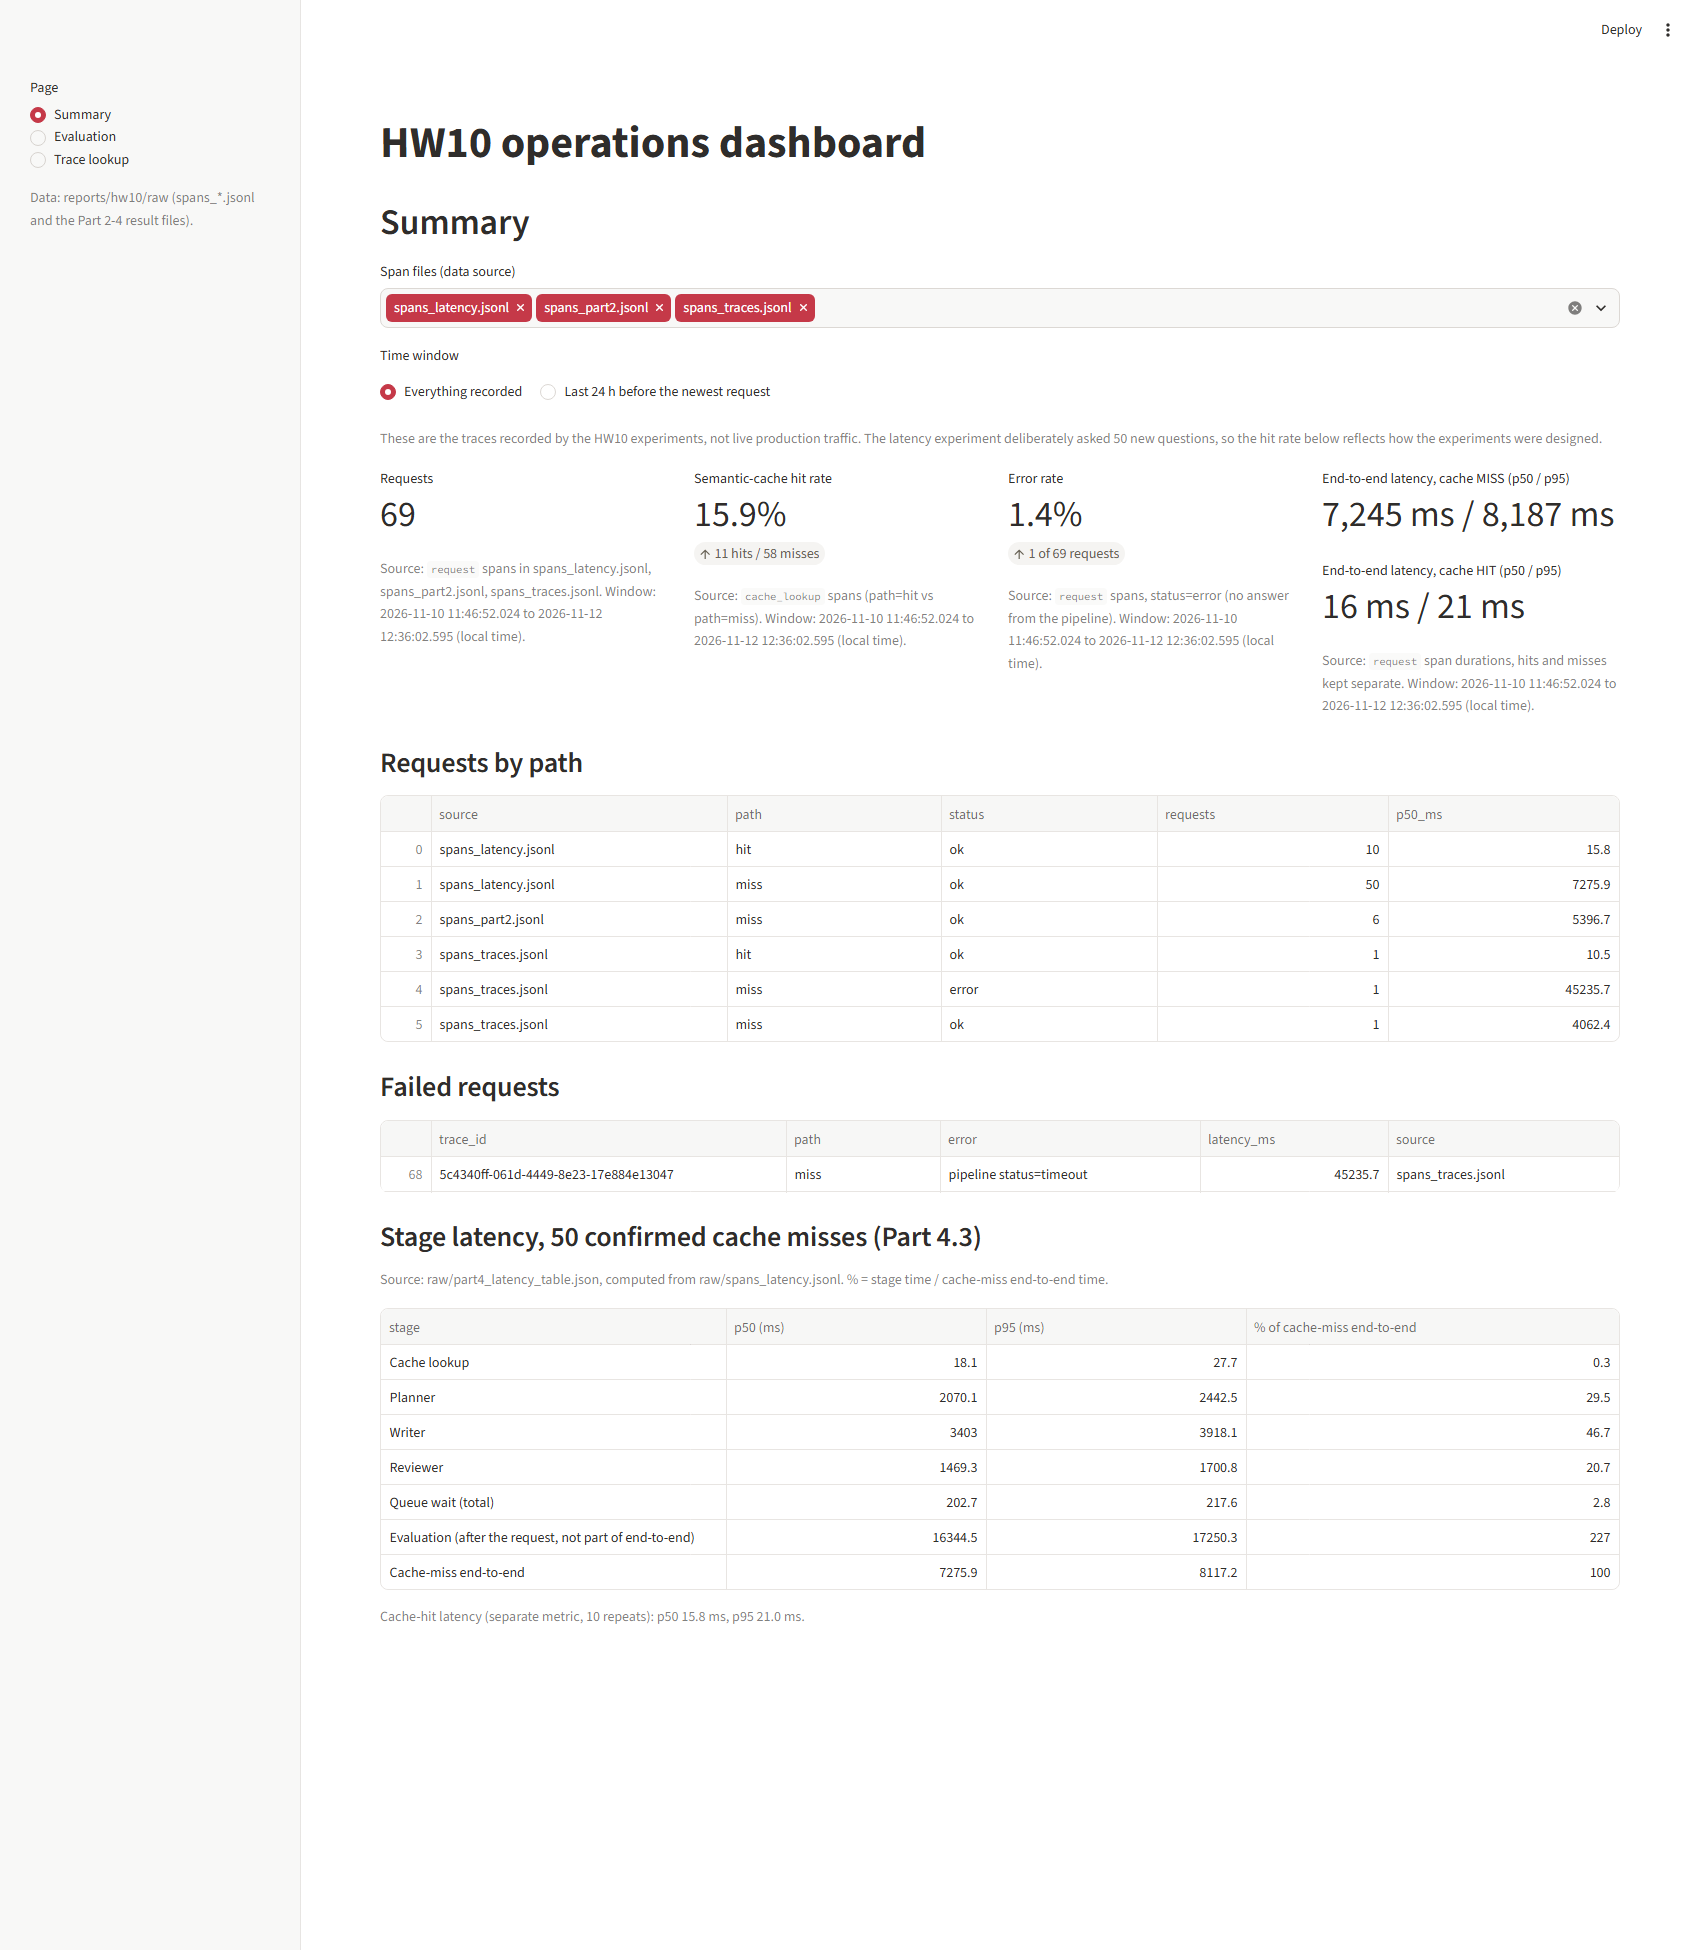
\includegraphics[width=0.97\linewidth,height=0.8\textheight,keepaspectratio]{screenshots/fig1_summary.png}\\[2pt]
\small \textit{Figure 1: Summary page: request count, cache hit rate, error rate and end-to-end latency, each with its data source and time window (all recorded runs).}
\end{center}
\begin{center}
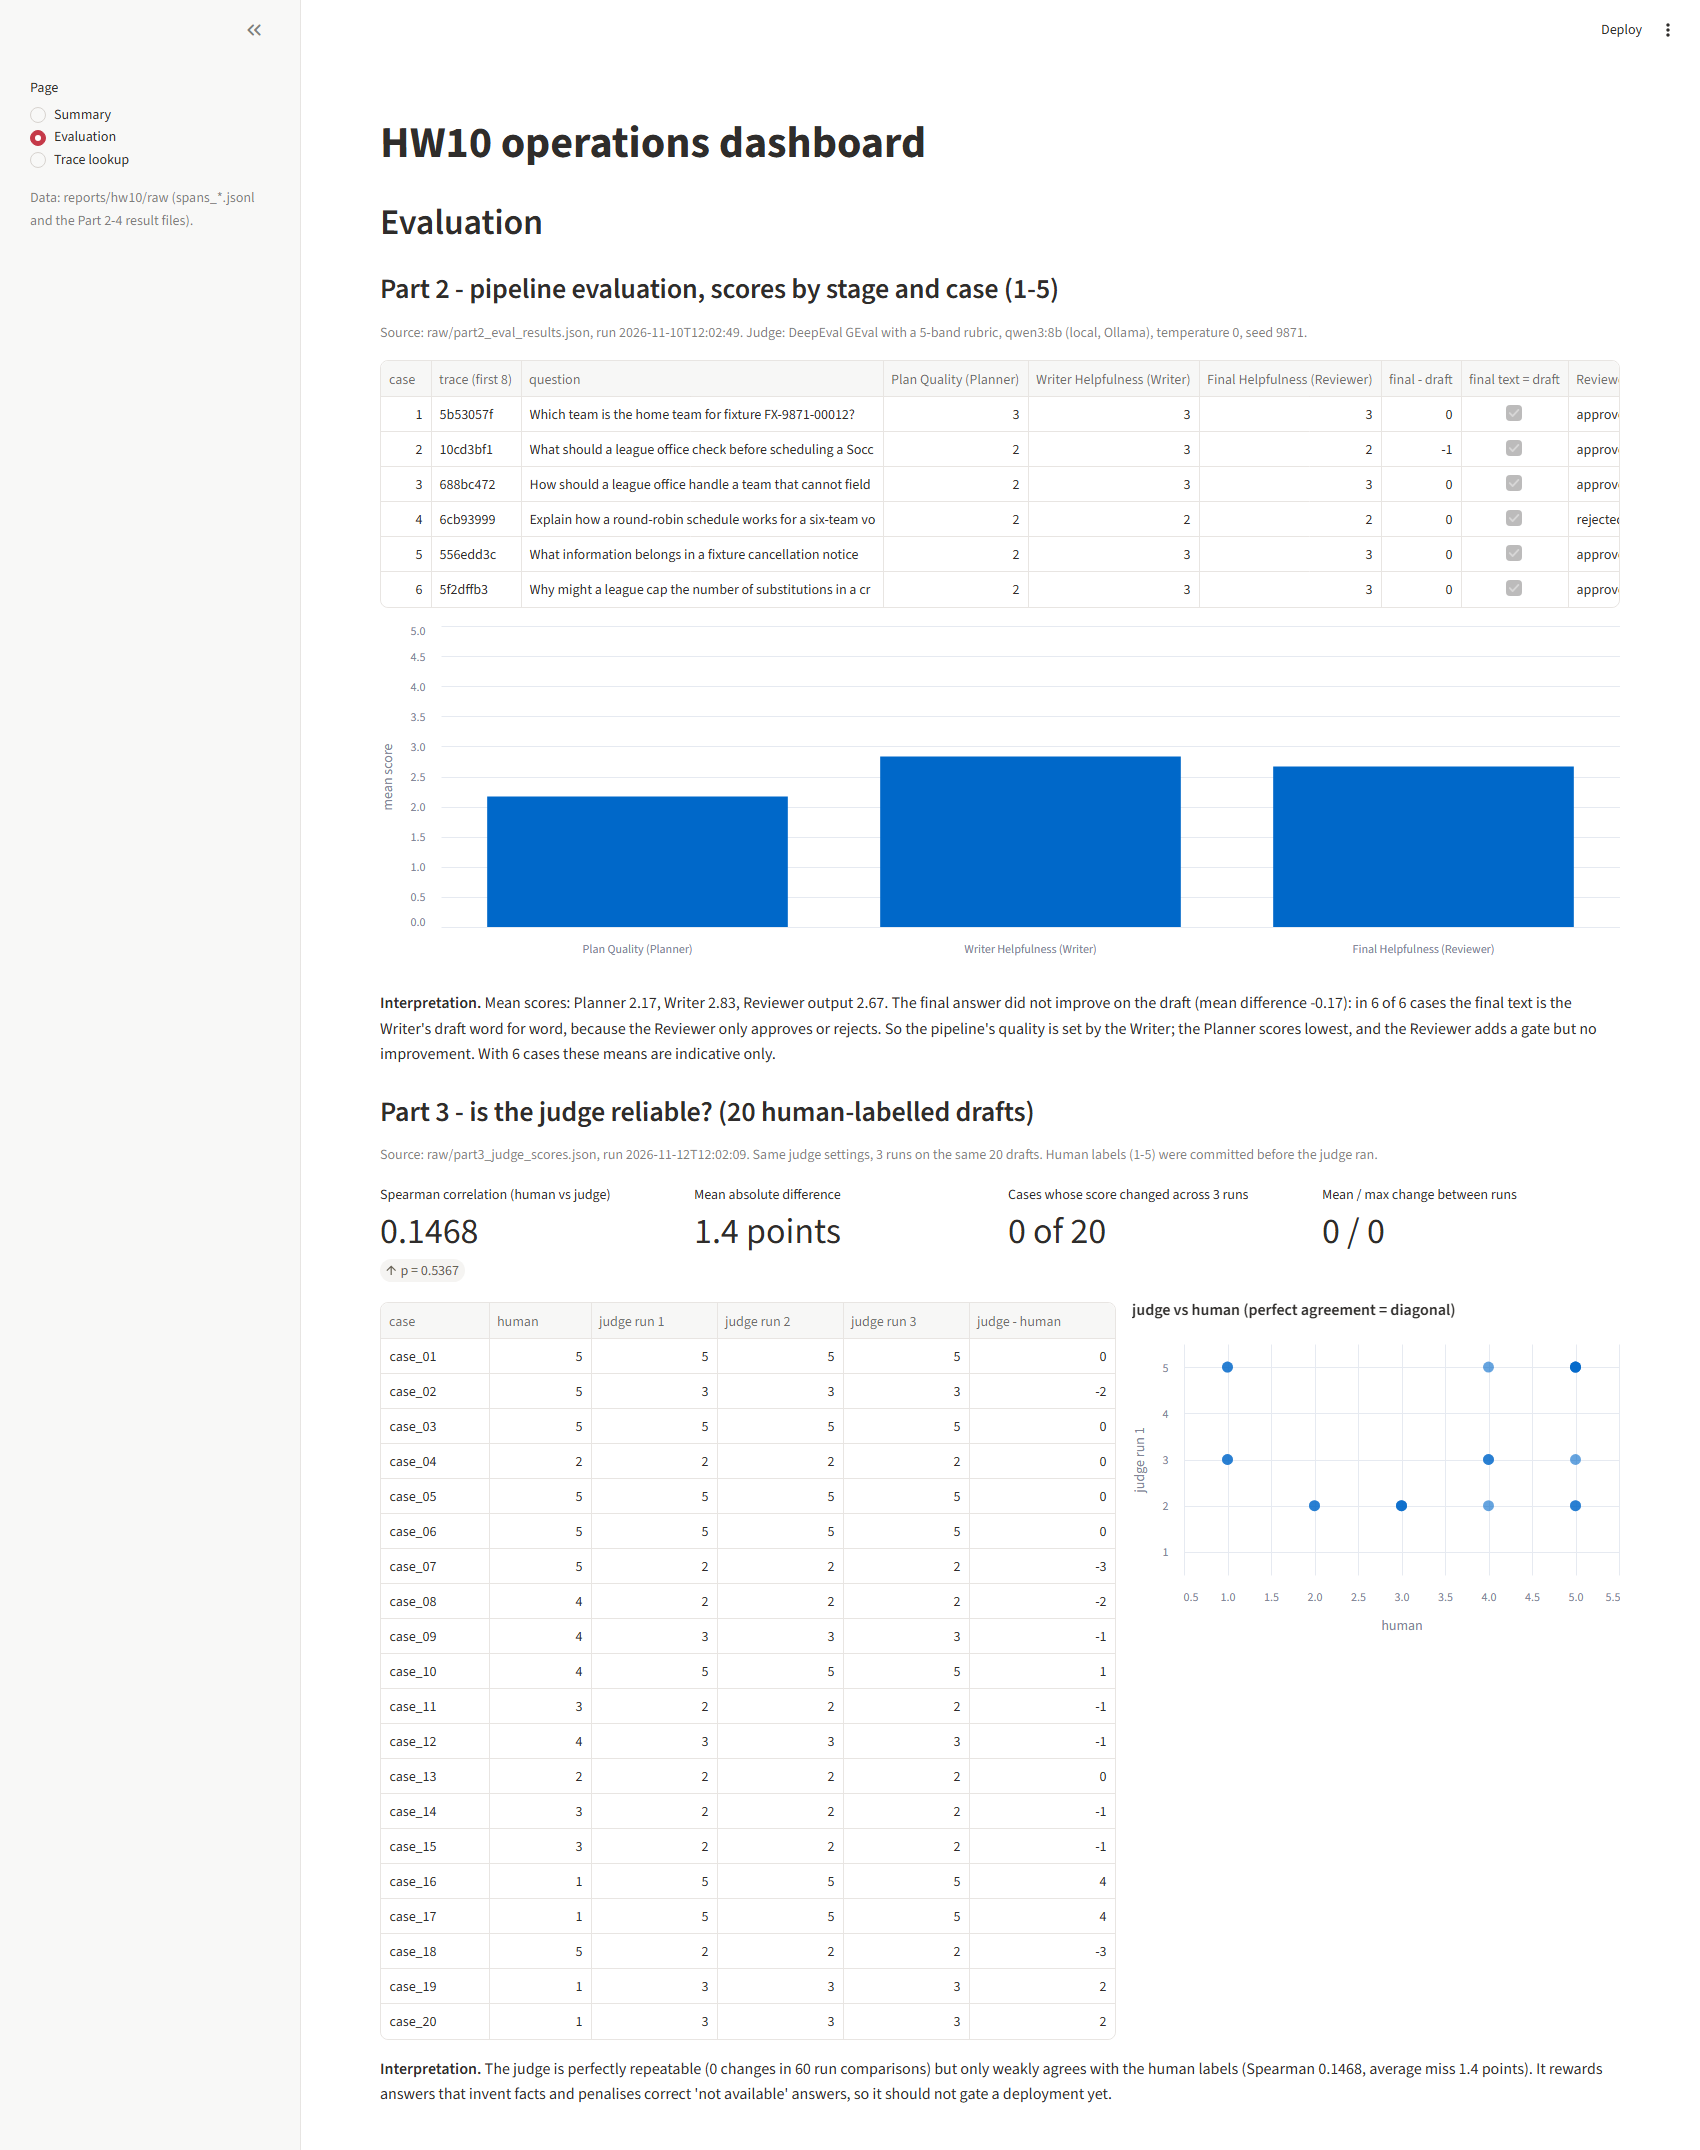
\includegraphics[width=0.97\linewidth,height=0.8\textheight,keepaspectratio]{screenshots/fig2_evaluation.png}\\[2pt]
\small \textit{Figure 2: Evaluation page: Part 2 scores by stage and case with the interpretation, and the Part 3 judge validation (Spearman, mean absolute difference, repeatability).}
\end{center}
\begin{center}
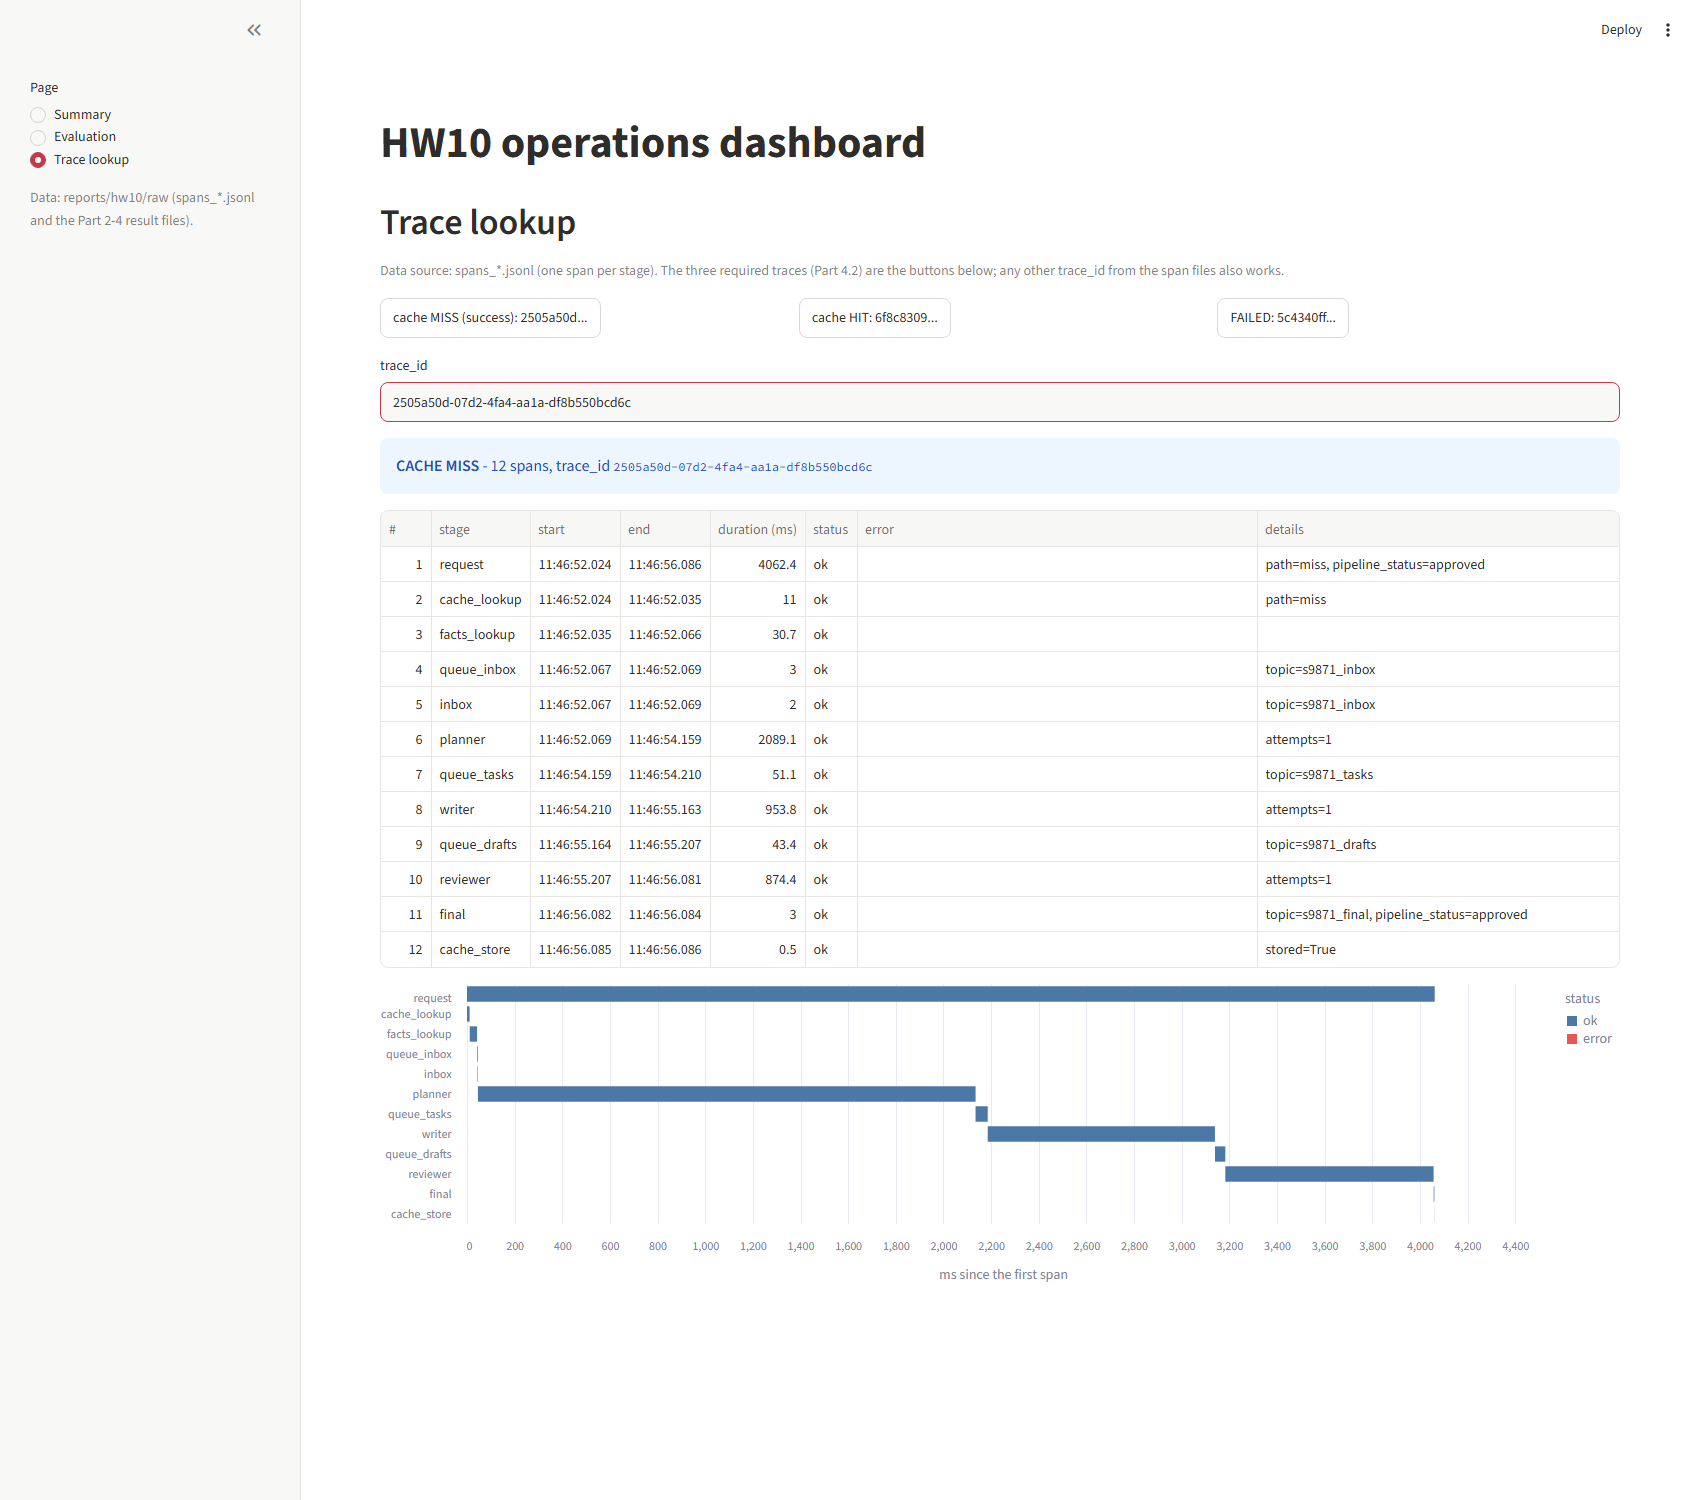
\includegraphics[width=0.97\linewidth,height=0.62\textheight,keepaspectratio]{screenshots/fig3_trace_cache_miss_2505a50d.png}\\[2pt]
\small \textit{Figure 3: Trace lookup page, cache MISS (success), trace\textbackslash{}\_\allowbreak{}id 2505a50d-07d2-4fa4-aa1a-df8b550bcd6c.}
\end{center}
\begin{center}
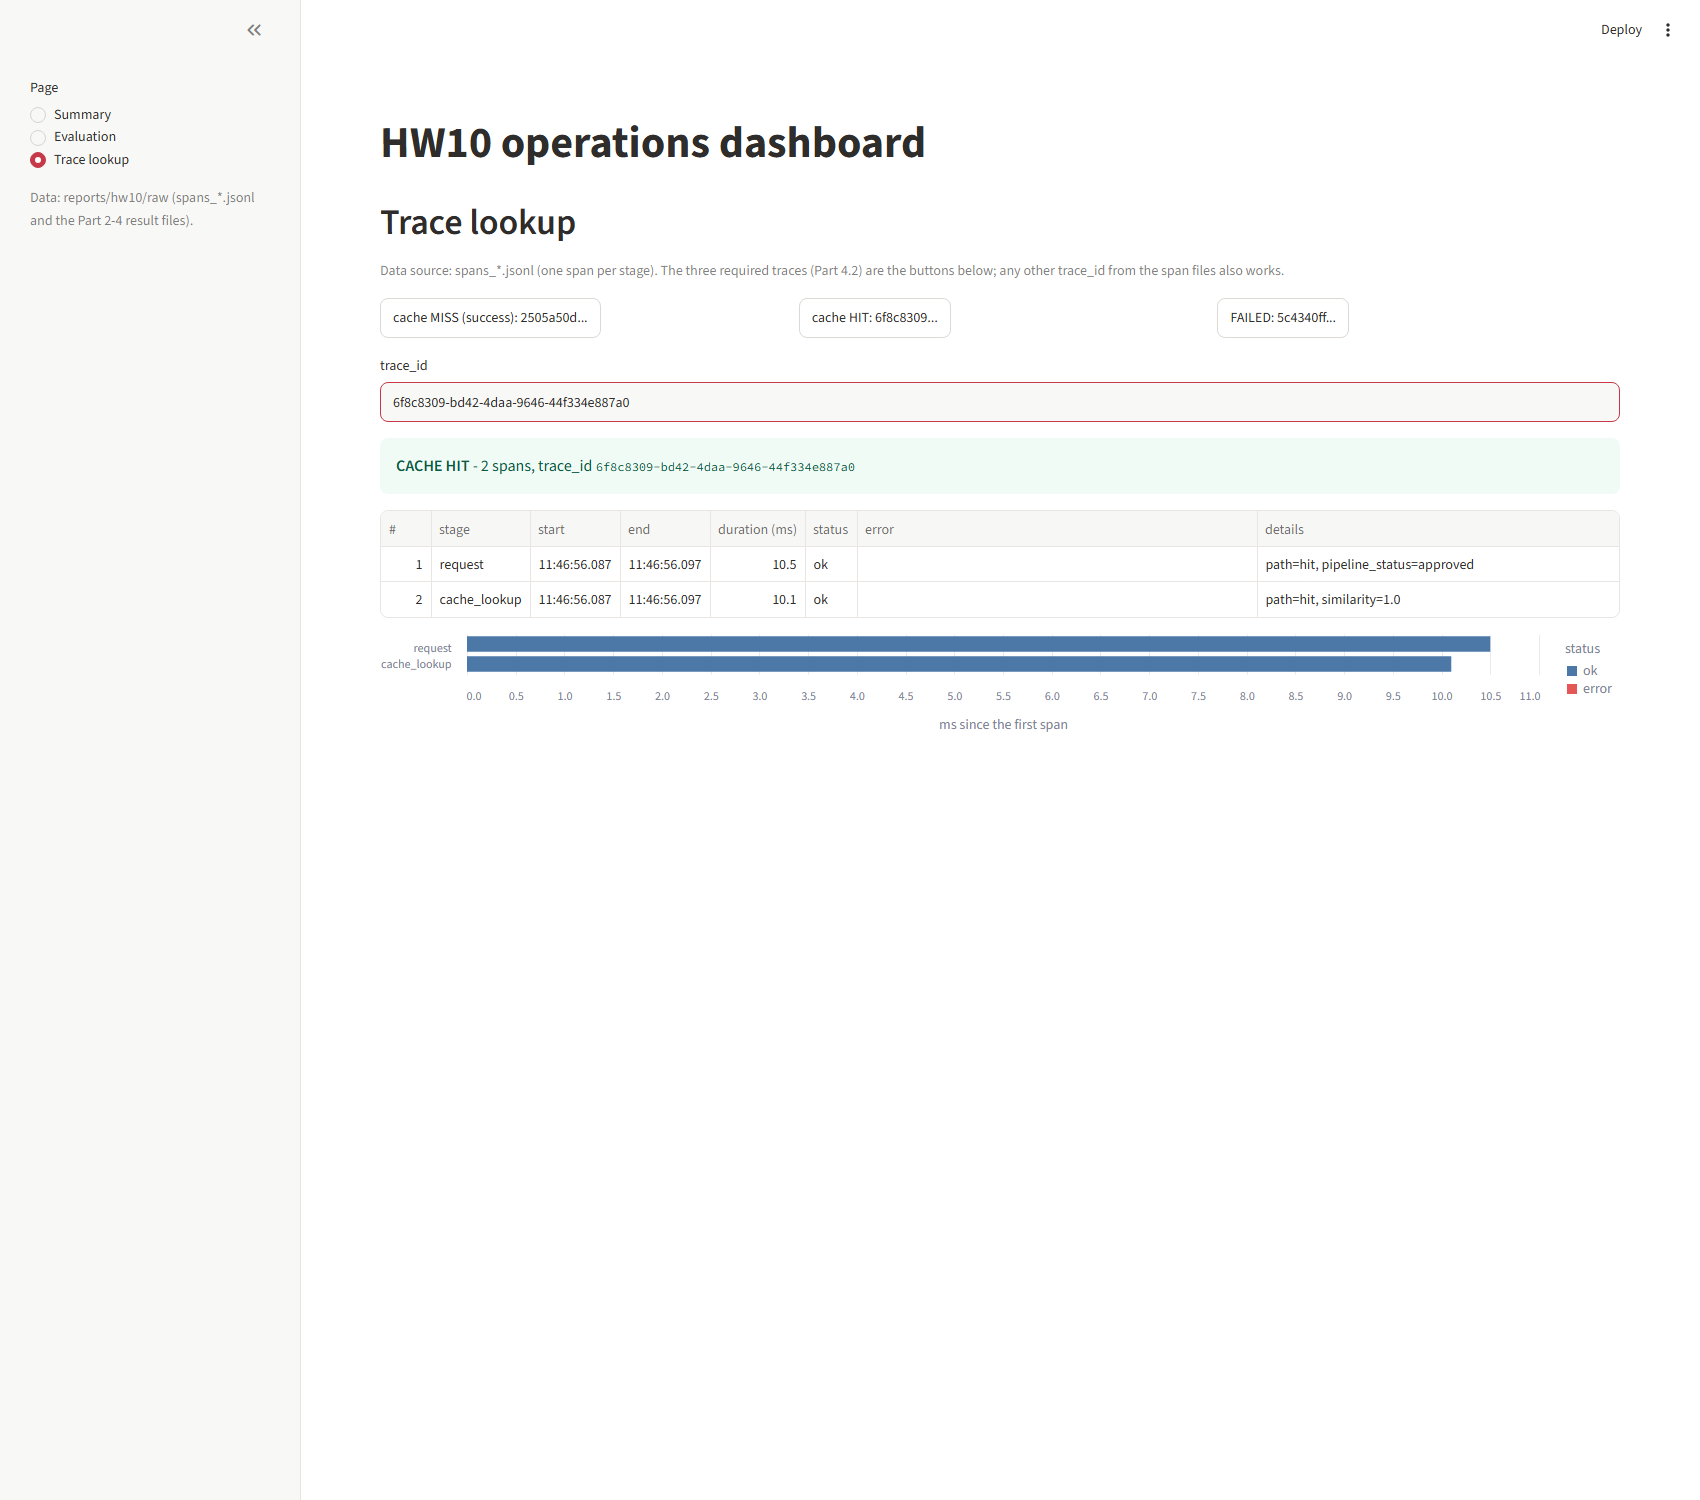
\includegraphics[width=0.97\linewidth,height=0.4\textheight,keepaspectratio]{screenshots/fig4_trace_cache_hit_6f8c8309.png}\\[2pt]
\small \textit{Figure 4: Trace lookup page, cache HIT, trace\textbackslash{}\_\allowbreak{}id 6f8c8309-bd42-4daa-9646-44f334e887a0.}
\end{center}
\begin{center}
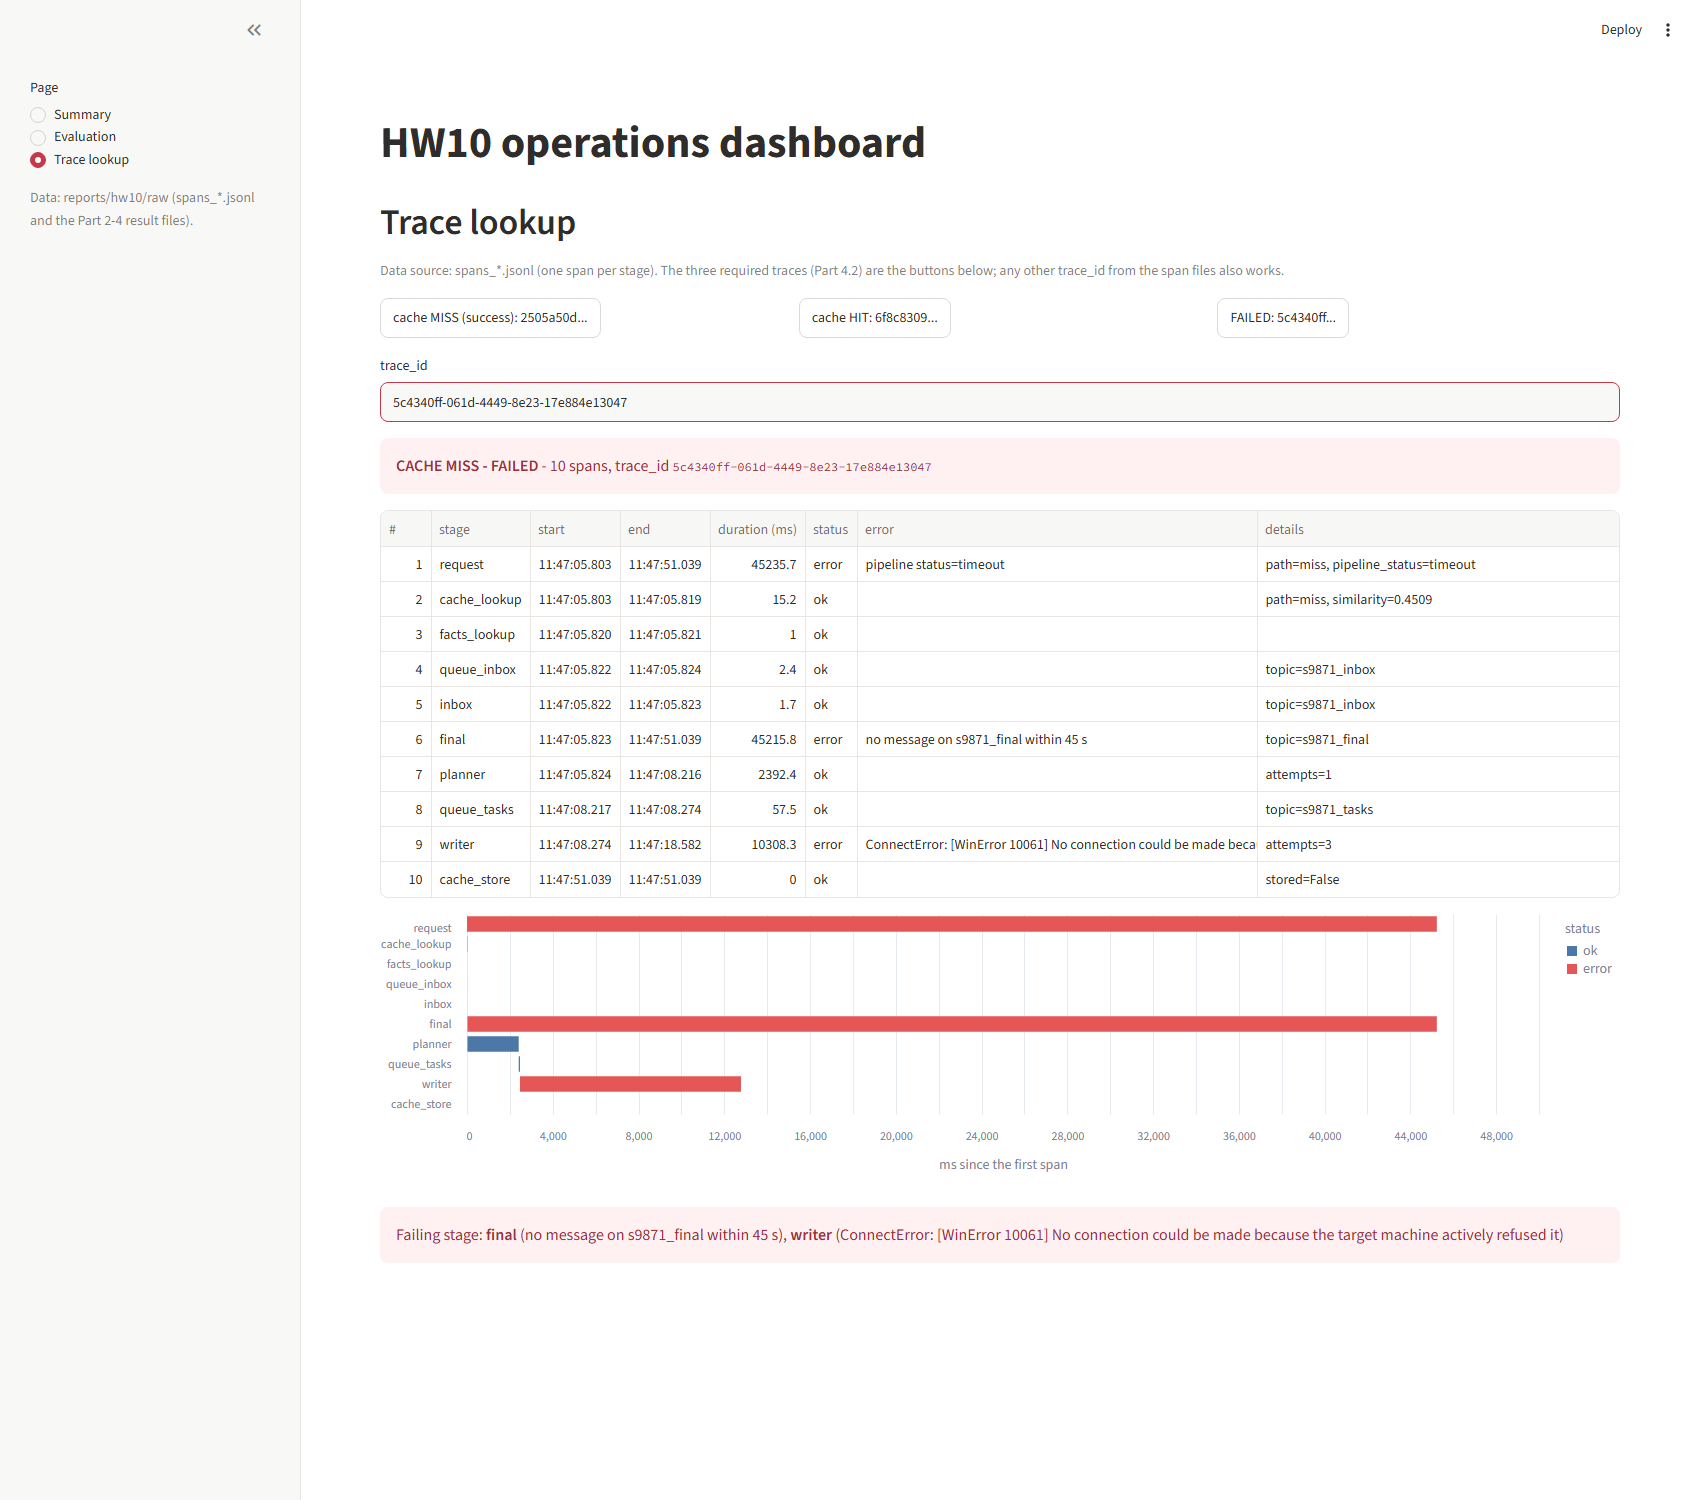
\includegraphics[width=0.97\linewidth,height=0.62\textheight,keepaspectratio]{screenshots/fig5_trace_failed_5c4340ff.png}\\[2pt]
\small \textit{Figure 5: Trace lookup page, FAILED request, trace\textbackslash{}\_\allowbreak{}id 5c4340ff-061d-4449-8e23-17e884e13047: failing stage writer.}
\end{center}
\section*{Part 2 -- Automated Evaluation of the Kafka Pipeline}
\subsection*{2.1 Inputs, linkage and the judge}
\texttt{evaluator.collect} reads the plan (\texttt{s9871\_\allowbreak{}tasks}), the draft (\texttt{s9871\_\allowbreak{}drafts}) and the final answer (\texttt{s9871\_\allowbreak{}final}) from Kafka and joins them on \texttt{correlation\_\allowbreak{}id}; it keeps each original message with its topic, partition, offset and timestamp. It stops at a deadline and skips malformed messages, and a request with a missing message is marked \texttt{incomplete}. The judge is DeepEval \textbf{GEval} with a local qwen3:8b (\texttt{judge.py}): temperature 0, seed 9871, thinking off, JSON-schema replies and a 120 s timeout per call, so an unavailable judge gives \texttt{judge\_\allowbreak{}unavailable} instead of hanging. GEval asks for 0-10 against a five-band rubric; the bands 0-2, 3-4, 5-6, 7-8, 9-10 are read back as 1-5 (1 = very poor, 5 = excellent). The same scale is used for the human labels in Part 3.

\begingroup\lstset{basicstyle=\ttfamily\tiny}
\begin{lstlisting}
def make_metric(key: str, judge: DeepEvalBaseLLM) -> GEval:
    name, criteria, params = CRITERIA[key]
    rubric = [Rubric(score_range=rng, expected_outcome=text) for rng, text in BANDS]
    return GEval(name=name, criteria=criteria, evaluation_params=params, rubric=rubric, model=judge, async_mode=False, threshold=0.5)

def band_to_score(raw_0_1: float) -> int:
    """GEval's 0-1 value (judge's 0-10 integer / 10) -> the 1-5 scale via the rubric bands."""
    s = round(raw_0_1 * 10)
    return 1 + (s >= 3) + (s >= 5) + (s >= 7) + (s >= 9)

CRITERIA = {
    "plan_quality": ("Plan Quality",
                     "Judge whether the Planner's three steps form a useful plan for answering the question: relevant to the question, specific, "
                     "complete enough to answer it, and in a sensible order.",
                     [SingleTurnParams.INPUT, SingleTurnParams.ACTUAL_OUTPUT]),
    "writer_helpfulness": ("Writer Helpfulness",
                           "Judge whether the Writer's draft answers the question accurately and usefully. Penalise answers that are wrong, "
                           "evasive, off-topic or that invent facts the question did not supply.",
                           [SingleTurnParams.INPUT, SingleTurnParams.ACTUAL_OUTPUT]),
    "final_helpfulness": ("Final Answer Helpfulness",
                          "Judge whether the final answer is helpful and relevant to the question: it must answer what was asked, be clear, "
                          "and not invent facts.",
                          [SingleTurnParams.INPUT, SingleTurnParams.ACTUAL_OUTPUT]),
}
\end{lstlisting}
\endgroup
\begingroup\lstset{basicstyle=\ttfamily\tiny}
\begin{lstlisting}
def collect(trace_ids: set[str], timeout_s: float = 60.0) -> tuple[dict, dict]:
    """-> ({trace_id: {"plan": rec, "draft": rec, "final": rec}}, stats). rec = {"value": parsed message, "topic", "partition", "offset", "timestamp_ms"}."""
    consumer = Consumer({"bootstrap.servers": BOOTSTRAP, "group.id": f"hw10-eval-{uuid.uuid4().hex[:8]}", "enable.auto.commit": False,
                         "auto.offset.reset": "earliest"})
    found: dict[str, dict] = {t: {} for t in trace_ids}
    stats = {"messages_read": 0, "malformed_skipped": 0, "timed_out": False}
    try:
        meta = consumer.list_topics(timeout=15).topics
        consumer.assign([TopicPartition(t, p, 0) for t in KINDS for p in meta[t].partitions])
        deadline = time.time() + timeout_s
        while time.time() < deadline and not all(len(v) == 3 for v in found.values()):
            msg = consumer.poll(1.0)
            if msg is None or msg.error():
                continue
            stats["messages_read"] += 1
            try:
                value = json.loads(msg.value())
                corr = value["correlation_id"]
            except (ValueError, KeyError, TypeError):
                stats["malformed_skipped"] += 1
                continue
            if corr in found:
                found[corr][KINDS[msg.topic()]] = {"value": value, "topic": msg.topic(), "partition": msg.partition(), "offset": msg.offset(),
                                                   "timestamp_ms": msg.timestamp()[1]}
        stats["timed_out"] = not all(len(v) == 3 for v in found.values())
    finally:
        consumer.close()
    return found, stats
\end{lstlisting}
\endgroup
\subsection*{2.2 The four criteria}
Plan Quality (score and reason), Writer Helpfulness (score and trace\textbackslash{}\_\allowbreak{}id), Final Answer Helpfulness (score and final answer) and Final-vs-Draft Improvement (both scores, the difference and an interpretation) are computed in \texttt{evaluator.evaluate}:

\begingroup\lstset{basicstyle=\ttfamily\tiny}
\begin{lstlisting}
def evaluate(trace_id: str, bundle: dict, judge: jd.DeepEvalBaseLLM, model_name: str = jd.JUDGE_MODEL) -> dict:
    """bundle = {"plan": rec, "draft": rec, "final": rec} from collect(); a missing piece makes the case "incomplete" (nothing is scored)."""
    t0 = tracing.now_ms()
    record = {"trace_id": trace_id, "status": "ok", "error": None, "judge": {"model": model_name, "temperature": jd.JUDGE_TEMPERATURE,
              "seed": jd.JUDGE_SEED, "scale": jd.SCALE}, "inputs": bundle}
    missing = [k for k in ("plan", "draft", "final") if k not in bundle]
    if missing:
        record.update(status="incomplete", error=f"missing {', '.join(missing)} message(s) for this correlation_id")
        tracing.emit(trace_id, "evaluation", t0, tracing.now_ms(), "error", record["error"])
        return record
    plan, draft, final = bundle["plan"]["value"], bundle["draft"]["value"], bundle["final"]["value"]
    question = draft.get("question") or plan.get("question", "")
    steps = "\n".join(f"{i}. {s}" for i, s in enumerate(plan.get("plan", []), 1))
    try:
        p = jd.score("plan_quality", judge, question, steps)
        w = jd.score("writer_helpfulness", judge, question, draft.get("draft", ""))
        f = jd.score("final_helpfulness", judge, question, final.get("answer", ""))
    except jd.JudgeUnavailable as exc:
        record.update(status="judge_unavailable", error=str(exc))
        tracing.emit(trace_id, "evaluation", t0, tracing.now_ms(), "error", str(exc))
        return record
    identical = draft.get("draft", "").strip() == final.get("answer", "").strip()
    record["scores"] = {
        "plan_quality": {"score": p["score"], "reason": p["reason"], "raw": p["raw"]},
        "writer_helpfulness": {"score": w["score"], "trace_id": trace_id, "reason": w["reason"], "raw": w["raw"]},
        "final_helpfulness": {"score": f["score"], "final_answer": final.get("answer", ""), "reason": f["reason"], "raw": f["raw"]},
        "final_vs_draft": {"draft_score": w["score"], "final_score": f["score"], "difference": f["score"] - w["score"], "final_equals_draft": identical,
                           "reviewer_status": final.get("status"), "interpretation": interpret(w["score"], f["score"], identical, final.get("status", ""))}}
    record["judge_ms"] = round(p["judge_ms"] + w["judge_ms"] + f["judge_ms"], 1)
    tracing.emit(trace_id, "evaluation", t0, tracing.now_ms(), judge_ms=record["judge_ms"], criteria=4)
    return record
\end{lstlisting}
\endgroup
One saved record (first request; the saved file also holds the full messages and every reason, long strings are cut here):

\begingroup\lstset{basicstyle=\ttfamily\tiny}
\begin{lstlisting}
{
 "trace_id": "5b53057f-2842-4932-834c-3d0e1ee4e1be",
 "status": "ok",
 "inputs": {
  "draft": {
   "value": {
    "question": "League database facts (authoritative; use them, do not invent other values):\n- FX-9871-00012: \"Strikers vs Bears (Volley...",
    "plan": [
     "Identify the fixture ID in the question (FX-9871-00012).",
     "Locate the home team information associated with the fixture ID in the database.",
     "Extract and report the home team name from the database entry."
    ],
    "draft": "The home team for fixture FX-9871-00012 is the Oakland Panthers.",
    "correlation_id": "5b53057f-2842-4932-834c-3d0e1ee4e1be"
   },
   "topic": "s9871_drafts",
   "partition": 0,
   "offset": 1,
   "timestamp_ms": 1794340856518
  },
  "final": {
   "value": {
    "status": "approved",
    "answer": "The home team for fixture FX-9871-00012 is the Oakland Panthers.",
    "review": "Answer correctly identifies the home team as specified in the database.",
    "correlation_id": "5b53057f-2842-4932-834c-3d0e1ee4e1be"
   },
   "topic": "s9871_final",
   "partition": 0,
   "offset": 1,
   "timestamp_ms": 1794340857735
  },
  "plan": {
   "value": {
    "question": "League database facts (authoritative; use them, do not invent other values):\n- FX-9871-00012: \"Strikers vs Bears (Volley...",
    "plan": [
     "Identify the fixture ID in the question (FX-9871-00012).",
     "Locate the home team information associated with the fixture ID in the database.",
     "Extract and report the home team name from the database entry."
    ],
    "correlation_id": "5b53057f-2842-4932-834c-3d0e1ee4e1be"
   },
   "topic": "s9871_tasks",
   "partition": 0,
   "offset": 0,
   "timestamp_ms": 1794340855367
  }
 },
 "scores": {
  "plan_quality": {
   "score": 3,
   "reason": "The steps are relevant, specific, and logically ordered, directly addressing the question by guiding the user to identif...",
   "raw": 0.5
  },
  "writer_helpfulness": {
   "score": 3,
   "trace_id": "5b53057f-2842-4932-834c-3d0e1ee4e1be",
   "reason": "The Actual Output correctly identifies the home team for fixture FX-9871-00012 as Oakland Panthers, which is explicitly ...",
   "raw": 0.5
  },
  "final_helpfulness": {
   "score": 3,
   "final_answer": "The home team for fixture FX-9871-00012 is the Oakland Panthers.",
   "reason": "The Actual Output directly answers the question by identifying the home team for the specified fixture. It is clear, con...",
   "raw": 0.5
  },
  "final_vs_draft": {
   "draft_score": 3,
   "final_score": 3,
   "difference": 0,
   "final_equals_draft": true,
   "reviewer_status": "approved",
   "interpretation": "The Reviewer returned the Writer's draft word for word (it only approves or rejects), so the final answer cannot be bett..."
  }
 }
}
\end{lstlisting}
\endgroup
Run at 2026-11-10T12:02:49 (local time). 6 of 6 requests evaluated (collect: 20 messages read, 0 malformed skipped). Judge: DeepEval GEval with a 5-band rubric, local qwen3:8b via Ollama, temperature 0, seed 9871, thinking off, 120 s timeout per call. Scale: 1 (very poor) to 5 (excellent). The judge sees the same question text the Planner saw (the database facts plus the question).

\begin{center}
{\scriptsize\setlength{\tabcolsep}{3pt}
\begin{tabular}{>{\raggedright\arraybackslash}p{0.25in}>{\raggedright\arraybackslash}p{1.5in}>{\raggedright\arraybackslash}p{0.6in}>{\raggedright\arraybackslash}p{0.55in}>{\raggedright\arraybackslash}p{0.7in}>{\raggedright\arraybackslash}p{0.7in}>{\raggedright\arraybackslash}p{0.45in}>{\raggedright\arraybackslash}p{0.5in}>{\raggedright\arraybackslash}p{0.6in}}
\toprule
\textbf{\#} & \textbf{question} & \textbf{trace} & \textbf{Plan Quality} & \textbf{Writer Helpfulness} & \textbf{Final Helpfulness} & \textbf{final - draft} & \textbf{final text = draft} & \textbf{Reviewer status} \\
\midrule
1 & Which team is the home team for fixture FX-9871-00012? & 5b53057f & 3 & 3 & 3 & +0 & yes & approved \\
2 & What should a league office check before scheduling a Soccer fixture o & 10cd3bf1 & 2 & 3 & 2 & -1 & yes & approved \\
3 & How should a league office handle a team that cannot field enough play & 688bc472 & 2 & 3 & 3 & +0 & yes & approved \\
4 & Explain how a round-robin schedule works for a six-team volleyball lea & 6cb93999 & 2 & 2 & 2 & +0 & yes & rejected \\
5 & What information belongs in a fixture cancellation notice sent to both & 556edd3c & 2 & 3 & 3 & +0 & yes & approved \\
6 & Why might a league cap the number of substitutions in a cricket match? & 5f2dffb3 & 2 & 3 & 3 & +0 & yes & approved \\
\bottomrule
\end{tabular}}
\end{center}
\begin{center}
{\small
\begin{tabular}{>{\raggedright\arraybackslash}p{3.6in}>{\raggedright\arraybackslash}p{1.5in}}
\toprule
\textbf{Stage} & \textbf{Mean score (1-5)} \\
\midrule
Plan Quality (Planner) & 2.17 \\
Writer Helpfulness (Writer draft) & 2.83 \\
Final Answer Helpfulness (Reviewer output) & 2.67 \\
Mean final - draft & -0.17 (min -1, max +0) \\
Requests where the final text is identical to the draft & 6 of 6 \\
\bottomrule
\end{tabular}}
\end{center}
What this shows: the final answer did not improve on the draft in any request (mean difference -0.17). The reason is structural, not a judge effect: the Reviewer does not rewrite, it only approves or rejects, so in 6 of 6 requests the final answer is the Writer's draft word for word. A non-zero difference on identical text is therefore judge variation between two differently worded criteria, not an improvement. The Planner's plans scored lowest (mean 2.17); in requests 3 to 6 (all scored 2) the judge's reasons say the steps are relevant but lack specificity or completeness. The judge is not perfectly consistent with itself: for request 2 its reason calls the plan specific, ordered and complete, yet the score is 2. Part 3 measures this judge against human labels. 6 requests is a small sample, so these means are indicative only.

Console output of \texttt{run\_\allowbreak{}part2.py} and \texttt{test\_\allowbreak{}evaluator.py} is in \texttt{RUN\_\allowbreak{}LOG.txt}; the evaluation spans (\texttt{evaluation}, same trace\textbackslash{}\_\allowbreak{}id) are in \texttt{raw/\allowbreak{}spans\_\allowbreak{}part2.jsonl}.

\section*{Part 3 -- Validating the Judge}
\subsection*{3.1 Frozen cases and human labels}
\texttt{eval\_\allowbreak{}cases.json} holds 20 real Writer drafts from the league pipeline (8 fixture-fact questions with database facts, including 2 fixture codes that do not exist, 7 general league questions and 5 questions the system has no data for); \texttt{human\_\allowbreak{}labels.csv} holds my own helpfulness label, 1-5, for each draft. Both were committed (commit \texttt{a03b38c}) before any judge score existed (the judge scores are in commit \texttt{5192512}); the labels were not changed afterwards. \texttt{verify\_\allowbreak{}hw10.py} checks the commit order and that both files are unchanged.

\begingroup\lstset{basicstyle=\ttfamily\tiny}
\begin{lstlisting}
case_01: Which team is the home team for fixture FX-9871-00012?
    draft: The home team for fixture FX-9871-00012 is the Oakland Panthers.
case_02: How many player spots are still open on fixture FX-9871-00031, and which teams are playing?
    draft: Fixture FX-9871-00031 has 22 player spots still open. The teams playing are the Milpitas Wolves and the Oakland Sharks.
case_03: Where will fixture FX-9871-00044 be played?
    draft: Fixture FX-9871-00044 will be played at Backesto Park in San Jose. The home team, San Jose Sharks, is listed as the host for this basketball match.
case_04: Name both teams in fixture FX-9871-00057 and say which one is at home.
    draft: The fixture FX-9871-00057 features the Fremont Tigers and Oakland Titans. The home team is the Fremont Tigers, playing at Northgate Park in Fremont.
    ... (20 cases in eval_cases.json)
\end{lstlisting}
\endgroup
\begingroup\lstset{basicstyle=\ttfamily\tiny}
\begin{lstlisting}
id,human_label | 01,5 | 02,5 | 03,5 | 04,2 | 05,5 | 06,5 | 07,5 | 08,4 | 09,4 | 10,4 | 11,3 | 12,4 | 13,2 | 14,3 | 15,3 | 16,1 | 17,1 | 18,5 | 19,1 | 20,1
\end{lstlisting}
\endgroup
\subsection*{3.2 and 3.3 Judge vs human, and repeatability}
The judge ran three times on the same 20 drafts with identical inputs and settings (\texttt{run\_\allowbreak{}part3.py}; per-case data for every run in \texttt{raw/\allowbreak{}part3\_\allowbreak{}judge\_\allowbreak{}scores.json} and \texttt{.csv}).

\begingroup\lstset{basicstyle=\ttfamily\tiny}
\begin{lstlisting}
def statistics(human: list[int], runs: list[list[int | None]]) -> dict:
    ok = [i for i in range(len(human)) if all(r[i] is not None for r in runs)]
    h = [human[i] for i in ok]
    rho, p = spearmanr(h, [runs[0][i] for i in ok])
    mad = [round(st.mean(abs(h[k] - r[i]) for k, i in enumerate(ok)), 3) for r in runs]
    changes = [abs(runs[a][i] - runs[b][i]) for a, b in itertools.combinations(range(len(runs)), 2) for i in ok]
    per_case = [max(r[i] for r in runs) - min(r[i] for r in runs) for i in ok]
    return {"n_scored": len(ok), "spearman_rho_run1": round(float(rho), 4), "spearman_p_run1": round(float(p), 4),
            "spearman_rho_per_run": [round(float(spearmanr(h, [r[i] for i in ok])[0]), 4) for r in runs],
            "mean_abs_difference_per_run": mad, "mean_abs_difference_run1": mad[0],
            "mean_judge_minus_mean_human_run1": round(st.mean(runs[0][i] for i in ok) - st.mean(h), 3),
            "exact_agreement_run1_pct": round(100 * sum(runs[0][i] == human[i] for i in ok) / len(ok), 1),
            "within_1_run1_pct": round(100 * sum(abs(runs[0][i] - human[i]) <= 1 for i in ok) / len(ok), 1),
            "cases_with_any_change_across_runs": sum(c > 0 for c in per_case), "cases_with_any_change_pct": round(100 * sum(c > 0 for c in per_case) / len(ok), 1),
            "pairwise_comparisons": len(changes), "pairwise_changed": sum(c > 0 for c in changes),
            "pairwise_changed_pct": round(100 * sum(c > 0 for c in changes) / len(changes), 1),
            "mean_abs_change": round(st.mean(changes), 4), "max_abs_change": max(changes)}
\end{lstlisting}
\endgroup
Run at 2026-11-12T12:02:09 (local time). Judge: Writer Helpfulness (GEval, 5-band rubric), local qwen3:8b, temperature 0, seed 9871, thinking off, scale 1 (very poor) to 5 (excellent). The 20 drafts (\texttt{eval\_\allowbreak{}cases.json}) and the human labels (\texttt{human\_\allowbreak{}labels.csv}) were committed before this run; their SHA-256 (line endings normalised) are 916e0bea895375a6... and 886be97023caa475... in \texttt{raw/\allowbreak{}part3\_\allowbreak{}judge\_\allowbreak{}scores.json}. The judge ran 3 times on the same inputs and settings.

\begin{center}
{\scriptsize\setlength{\tabcolsep}{3pt}
\begin{tabular}{>{\raggedright\arraybackslash}p{0.55in}>{\raggedright\arraybackslash}p{2.7in}>{\raggedright\arraybackslash}p{0.5in}>{\raggedright\arraybackslash}p{0.55in}>{\raggedright\arraybackslash}p{0.45in}>{\raggedright\arraybackslash}p{0.45in}>{\raggedright\arraybackslash}p{0.6in}}
\toprule
\textbf{case} & \textbf{question} & \textbf{human} & \textbf{judge run 1} & \textbf{run 2} & \textbf{run 3} & \textbf{judge - human (run 1)} \\
\midrule
case\_\allowbreak{}01 & Which team is the home team for fixture FX-9871-00012? & 5 & 5 & 5 & 5 & +0 \\
case\_\allowbreak{}02 & How many player spots are still open on fixture FX-9871-00031, & 5 & 3 & 3 & 3 & -2 \\
case\_\allowbreak{}03 & Where will fixture FX-9871-00044 be played? & 5 & 5 & 5 & 5 & +0 \\
case\_\allowbreak{}04 & Name both teams in fixture FX-9871-00057 and say which one is & 2 & 2 & 2 & 2 & +0 \\
case\_\allowbreak{}05 & Is there room for 3 more players to register for fixture FX-98 & 5 & 5 & 5 & 5 & +0 \\
case\_\allowbreak{}06 & What is the name of fixture FX-9871-00078? & 5 & 5 & 5 & 5 & +0 \\
case\_\allowbreak{}07 & Which team is the home team for fixture FX-9871-09101? & 5 & 2 & 2 & 2 & -3 \\
case\_\allowbreak{}08 & How many player spots are open on fixture FX-9871-09102? & 4 & 2 & 2 & 2 & -2 \\
case\_\allowbreak{}09 & What should a league office check before scheduling a Soccer f & 4 & 3 & 3 & 3 & -1 \\
case\_\allowbreak{}10 & How should a league office handle a team that cannot field eno & 4 & 5 & 5 & 5 & +1 \\
case\_\allowbreak{}11 & Explain how a round-robin schedule works for a six-team volley & 3 & 2 & 2 & 2 & -1 \\
case\_\allowbreak{}12 & What information belongs in a fixture cancellation notice sent & 4 & 3 & 3 & 3 & -1 \\
case\_\allowbreak{}13 & Why might a league cap the number of substitutions in a cricke & 2 & 2 & 2 & 2 & +0 \\
case\_\allowbreak{}14 & What are three ways to reduce no-shows for early-morning baske & 3 & 2 & 2 & 2 & -1 \\
case\_\allowbreak{}15 & How do you break a tie in league standings when two teams have & 3 & 2 & 2 & 2 & -1 \\
case\_\allowbreak{}16 & What was the final score of last season's championship game? & 1 & 5 & 5 & 5 & +4 \\
case\_\allowbreak{}17 & What is the phone number of the league office? & 1 & 5 & 5 & 5 & +4 \\
case\_\allowbreak{}18 & Which referee is assigned to fixture FX-9871-00012? & 5 & 2 & 2 & 2 & -3 \\
case\_\allowbreak{}19 & How much does it cost to register a team this season? & 1 & 3 & 3 & 3 & +2 \\
case\_\allowbreak{}20 & Summarise the weather forecast for this Saturday's fixtures. & 1 & 3 & 3 & 3 & +2 \\
\bottomrule
\end{tabular}}
\end{center}
\begin{center}
{\small
\begin{tabular}{>{\raggedright\arraybackslash}p{3.4in}>{\raggedright\arraybackslash}p{2.5in}}
\toprule
\textbf{Statistic} & \textbf{Value} \\
\midrule
Spearman rank correlation, human vs judge (run 1) & 0.1468 (p = 0.5367, n = 20) \\
Mean absolute difference, human vs judge & 1.4 / 1.4 / 1.4 (runs 1 / 2 / 3) \\
Mean judge score minus mean human label & -0.1 \\
Exact agreement / within 1 point (run 1) & 30.0\% / 60.0\% \\
Cases whose score changed across the 3 runs & 0 of 20 (0.0\%) \\
Run pairs where a score changed & 0 of 60 (0.0\%) \\
Mean / maximum absolute change between runs & 0 / 0 \\
\bottomrule
\end{tabular}}
\end{center}
What this shows: the judge is perfectly repeatable but weakly valid. Its scores did not change in any of the 60 run-to-run comparisons, which is expected with temperature 0 and a fixed seed, so this measures determinism, not robustness: it says nothing about how the score moves if the wording of the draft or the prompt changes. Agreement with the human labels is weak: Spearman 0.1468 (p = 0.5367, so not distinguishable from no correlation at n = 20) and an average miss of 1.4 points on a 5-point scale. The similar mean scores (difference -0.1) hide errors in both directions.

The errors are systematic. In 4 of the 6 drafts the human rated 1 or 2 (case\_\allowbreak{}16, case\_\allowbreak{}17, case\_\allowbreak{}19, case\_\allowbreak{}20), the judge rated 3 or higher: these are drafts that state a score, a phone number, a fee or a forecast that the system has no data for. The judge's reasons say the draft "directly addresses the question", so it rewards answering over being supported. In the other direction, 3 drafts the human rated 4 or 5 (case\_\allowbreak{}07, case\_\allowbreak{}08, case\_\allowbreak{}18) got 2 or lower: the judge penalised answers that correctly say the information does not exist or is not in the database.

Would I trust this judge to gate a deployment? No. A gate must catch unsupported answers, and this judge scores several invented answers higher than correct refusals. Evidence I would require first: (1) a Spearman correlation with human labels clearly above chance on a larger set (at least 100 labelled drafts, ideally labelled by more than one person so human-human agreement is known); (2) a criterion that checks the draft against the supplied facts, so that unsupported answers score low, then re-validated on the same labels; (3) a check of the judge under changes (paraphrased drafts, a different seed, a second judge model), since repeatability under a fixed seed is not robustness; (4) an agreed error budget, for example at most one unsupported answer in 20 passed by the gate. The labels were written by one person on 20 cases, so these statistics are indicative only.

\section*{Part 4 -- Distributed Tracing and Latency Analysis}
\subsection*{4.1 Trace propagation}
\texttt{trace\_\allowbreak{}id} is the HW8 \texttt{correlation\_\allowbreak{}id}: \texttt{CachedQA.ask} creates it, \texttt{PipelineClient.ask} uses it as the Kafka message key and \texttt{correlation\_\allowbreak{}id}, every agent copies it unchanged, and the evaluator reuses it. No second identifier exists. Every stage appends one structured JSON span to a span file (\texttt{tracing.emit}; a no-op unless \texttt{HW10\_\allowbreak{}SPANS} is set, so HW8 and HW9 behave as before):

\begingroup\lstset{basicstyle=\ttfamily\tiny}
\begin{lstlisting}
def emit(trace_id: str | None, stage: str, start_ms: float, end_ms: float, status: str = "ok", error: str | None = None, **attrs) -> dict | None:
    path = os.environ.get("HW10_SPANS")
    if not path or not trace_id:
        return None
    span = {"trace_id": trace_id, "stage": stage, "start": iso(start_ms), "end": iso(end_ms), "start_ms": round(start_ms, 1),
            "end_ms": round(end_ms, 1), "duration_ms": round(end_ms - start_ms, 1), "status": status, "error": error, "attrs": attrs}
    fd = os.open(path, os.O_WRONLY | os.O_APPEND | os.O_CREAT, 0o644)
    try:
        os.write(fd, (json.dumps(span, ensure_ascii=False) + "\n").encode("utf-8"))
    finally:
        os.close(fd)
    return span
\end{lstlisting}
\endgroup
Each agent records its queue wait and its own span inside the shared consume-handle-produce loop (\texttt{run\_\allowbreak{}stage}), and the ingress records the cache lookup, the inbox publish and the final answer:

\begingroup\lstset{basicstyle=\ttfamily\tiny}
\begin{lstlisting}
        t_start = tracing.now_ms()
        sent_at = tracing.kafka_ms(msg)
        if sent_at is not None:  # HW10 tracing: time the message sat in the topic before this stage picked it up
            tracing.emit(corr, f"queue_{in_topic.split('_', 1)[1]}", sent_at, t_start, topic=in_topic, partition=msg.partition(), offset=msg.offset())        ...
        if out is not None or error:
            tracing.emit(corr, stage, t_start, tracing.now_ms(), "ok" if out is not None else "error", None if out is not None else error,
                         attempts=attempt, instance=INSTANCE or None)
\end{lstlisting}
\endgroup
\begingroup\lstset{basicstyle=\ttfamily\tiny}
\begin{lstlisting}
        w_lookup_end = tracing.now_ms()
        similarity = best["similarity"] if best else None
        ...
        is_hit = bool(best and similarity >= threshold and not stale)
        tracing.emit(trace_id, "cache_lookup", w0, w_lookup_end, path="hit" if is_hit else "miss", similarity=similarity, threshold=threshold,
                     embed_ms=round(timings["embed_ms"], 1), search_ms=round(timings["search_ms"], 1), stale=stale)
\end{lstlisting}
\endgroup
One real span (the Planner of the miss trace below):

\begingroup\lstset{basicstyle=\ttfamily\tiny}
\begin{lstlisting}
{
 "trace_id": "2505a50d-07d2-4fa4-aa1a-df8b550bcd6c",
 "stage": "planner",
 "start": "2026-11-10T11:46:52.069",
 "end": "2026-11-10T11:46:54.159",
 "start_ms": 1794340012070.0,
 "end_ms": 1794340014159.1,
 "duration_ms": 2089.1,
 "status": "ok",
 "error": null,
 "attrs": {
  "attempts": 1,
  "instance": null
 }
}
\end{lstlisting}
\endgroup
\subsection*{4.2 The three required traces}
One identifier per request: the \texttt{trace\_\allowbreak{}id} of every span is the HW8 \texttt{correlation\_\allowbreak{}id} (the same value is in the Kafka messages), so nothing is joined afterwards. Each stage writes one JSON span with trace\_\allowbreak{}id, stage, start, end, status and error (\texttt{code/\allowbreak{}kafka\_\allowbreak{}hw8/\allowbreak{}tracing.py}; the spans of all three traces are in \texttt{raw/\allowbreak{}spans\_\allowbreak{}traces.jsonl}). \texttt{queue\_\allowbreak{}*} spans are the time a message waited in a topic before the next stage took it (from the Kafka message timestamp); \texttt{final} is the ingress receiving the Reviewer's answer; \texttt{request} is the whole request.

\subsection*{Cache MISS, successful - trace\_\allowbreak{}id 2505a50d-07d2-4fa4-aa1a-df8b550bcd6c}
Question: Which team is the home team for fixture FX-9871-00012?

\begin{center}
{\scriptsize\setlength{\tabcolsep}{3pt}
\begin{tabular}{>{\raggedright\arraybackslash}p{0.2in}>{\raggedright\arraybackslash}p{1.0in}>{\raggedright\arraybackslash}p{0.85in}>{\raggedright\arraybackslash}p{0.85in}>{\raggedright\arraybackslash}p{0.8in}>{\raggedright\arraybackslash}p{0.45in}>{\raggedright\arraybackslash}p{1.7in}}
\toprule
\textbf{\#} & \textbf{stage} & \textbf{start} & \textbf{end} & \textbf{duration (ms)} & \textbf{status} & \textbf{error / details} \\
\midrule
1 & request & 11:46:52.024 & 11:46:56.086 & 4,062.4 & ok & path=miss, pipeline\_\allowbreak{}status=approved \\
2 & cache\_\allowbreak{}lookup & 11:46:52.024 & 11:46:52.035 & 11.0 & ok & path=miss \\
3 & facts\_\allowbreak{}lookup & 11:46:52.035 & 11:46:52.066 & 30.7 & ok &  \\
4 & queue\_\allowbreak{}inbox & 11:46:52.067 & 11:46:52.069 & 3.0 & ok &  \\
5 & inbox & 11:46:52.067 & 11:46:52.069 & 2.0 & ok &  \\
6 & planner & 11:46:52.069 & 11:46:54.159 & 2,089.1 & ok & attempts=1 \\
7 & queue\_\allowbreak{}tasks & 11:46:54.159 & 11:46:54.210 & 51.1 & ok &  \\
8 & writer & 11:46:54.210 & 11:46:55.163 & 953.8 & ok & attempts=1 \\
9 & queue\_\allowbreak{}drafts & 11:46:55.164 & 11:46:55.207 & 43.4 & ok &  \\
10 & reviewer & 11:46:55.207 & 11:46:56.081 & 874.4 & ok & attempts=1 \\
11 & final & 11:46:56.082 & 11:46:56.084 & 3.0 & ok & pipeline\_\allowbreak{}status=approved \\
12 & cache\_\allowbreak{}store & 11:46:56.085 & 11:46:56.086 & 0.5 & ok & stored=True \\
\bottomrule
\end{tabular}}
\end{center}
\subsection*{Cache HIT - trace\_\allowbreak{}id 6f8c8309-bd42-4daa-9646-44f334e887a0}
Question: Which team is the home team for fixture FX-9871-00012? (the same question asked again)

\begin{center}
{\scriptsize\setlength{\tabcolsep}{3pt}
\begin{tabular}{>{\raggedright\arraybackslash}p{0.2in}>{\raggedright\arraybackslash}p{1.0in}>{\raggedright\arraybackslash}p{0.85in}>{\raggedright\arraybackslash}p{0.85in}>{\raggedright\arraybackslash}p{0.8in}>{\raggedright\arraybackslash}p{0.45in}>{\raggedright\arraybackslash}p{1.7in}}
\toprule
\textbf{\#} & \textbf{stage} & \textbf{start} & \textbf{end} & \textbf{duration (ms)} & \textbf{status} & \textbf{error / details} \\
\midrule
1 & request & 11:46:56.087 & 11:46:56.097 & 10.5 & ok & path=hit, pipeline\_\allowbreak{}status=approved \\
2 & cache\_\allowbreak{}lookup & 11:46:56.087 & 11:46:56.097 & 10.1 & ok & path=hit, similarity=1.0 \\
\bottomrule
\end{tabular}}
\end{center}
\subsection*{FAILED - trace\_\allowbreak{}id 5c4340ff-061d-4449-8e23-17e884e13047}
Question: How many open player slots are left on fixture FX-9871-00031?. The Writer process was replaced by one whose model endpoint was unreachable (OLLAMA\_\allowbreak{}HOST pointed at a closed port), so a real failure was produced rather than a simulated one.

\begin{center}
{\scriptsize\setlength{\tabcolsep}{3pt}
\begin{tabular}{>{\raggedright\arraybackslash}p{0.2in}>{\raggedright\arraybackslash}p{1.0in}>{\raggedright\arraybackslash}p{0.85in}>{\raggedright\arraybackslash}p{0.85in}>{\raggedright\arraybackslash}p{0.8in}>{\raggedright\arraybackslash}p{0.45in}>{\raggedright\arraybackslash}p{1.7in}}
\toprule
\textbf{\#} & \textbf{stage} & \textbf{start} & \textbf{end} & \textbf{duration (ms)} & \textbf{status} & \textbf{error / details} \\
\midrule
1 & request & 11:47:05.803 & 11:47:51.039 & 45,235.7 & error & pipeline status=timeout \\
2 & cache\_\allowbreak{}lookup & 11:47:05.803 & 11:47:05.819 & 15.2 & ok & path=miss, similarity=0.4509 \\
3 & facts\_\allowbreak{}lookup & 11:47:05.820 & 11:47:05.821 & 1.0 & ok &  \\
4 & queue\_\allowbreak{}inbox & 11:47:05.822 & 11:47:05.824 & 2.4 & ok &  \\
5 & inbox & 11:47:05.822 & 11:47:05.823 & 1.7 & ok &  \\
6 & final & 11:47:05.823 & 11:47:51.039 & 45,215.8 & error & no message on s9871\_\allowbreak{}final within 45 s \\
7 & planner & 11:47:05.824 & 11:47:08.216 & 2,392.4 & ok & attempts=1 \\
8 & queue\_\allowbreak{}tasks & 11:47:08.217 & 11:47:08.274 & 57.5 & ok &  \\
9 & writer & 11:47:08.274 & 11:47:18.582 & 10,308.3 & error & ConnectError: [WinError 10061] No connection could be made because the target machine actively refused it \\
10 & cache\_\allowbreak{}store & 11:47:51.039 & 11:47:51.039 & 0.0 & ok & stored=False \\
\bottomrule
\end{tabular}}
\end{center}
What this shows: the hit trace has only \texttt{cache\_\allowbreak{}lookup} (path=hit, 10.1 ms) and the \texttt{request} span; no Kafka stage runs. The miss trace has every stage in order (cache\_\allowbreak{}lookup, facts\_\allowbreak{}lookup, inbox, planner, writer, reviewer, final, cache\_\allowbreak{}store) with 3 queue-wait spans between the agents. In the failed trace the failing stage is \textbf{writer}: three attempts, error \texttt{ConnectError:\allowbreak{} [WinError 10061] No connection could be made because the target machine actively refused it}, after which the message was dead-lettered; the ingress then found no answer on the final topic within 45 s, so \texttt{final} and \texttt{request} carry the status error too, and nothing was cached. The trace identifies where it failed (writer) and the symptom the caller saw (no answer), which the single \texttt{request} span would not.

\subsection*{4.3 Stage-latency experiment}
\texttt{run\_\allowbreak{}latency.py}: 50 requests through the real system, one at a time, against an empty semantic cache. Each request counts only if the response said \texttt{is\_\allowbreak{}cached=False} \textbf{and} its \texttt{cache\_\allowbreak{}lookup} span said \texttt{path=miss}; a question the cache happened to answer would have been skipped and replaced from the pool in \texttt{latency\_\allowbreak{}questions.py} (none was). The judge then evaluated the 50 requests in a separate pass so it did not share the GPU with the pipeline being timed. Percentages use the sum of a stage's time over the 50 requests divided by the sum of their end-to-end (\texttt{request} span) times.

Run at 2026-11-12T12:49:42 (local time), one request at a time, empty semantic cache, threshold 0.85. All 50 requests were confirmed misses: the response said is\_\allowbreak{}cached=False and the trace's cache\_\allowbreak{}lookup span said path=miss (0 pool questions were skipped because the cache answered them). Source: \texttt{raw/\allowbreak{}spans\_\allowbreak{}latency.jsonl} (one JSON span per stage and trace\_\allowbreak{}id).

\begin{center}
{\small
\begin{tabular}{>{\raggedright\arraybackslash}p{3.0in}>{\raggedright\arraybackslash}p{0.9in}>{\raggedright\arraybackslash}p{0.9in}>{\raggedright\arraybackslash}p{1.2in}}
\toprule
\textbf{Stage} & \textbf{p50 (ms)} & \textbf{p95 (ms)} & \textbf{\% of cache-miss end-to-end} \\
\midrule
Cache lookup & 18.1 & 27.7 & 0.3\% \\
Planner & 2,070.1 & 2,442.5 & 29.5\% \\
Writer & 3,403.0 & 3,918.1 & 46.7\% \\
Reviewer & 1,469.3 & 1,700.8 & 20.7\% \\
Queue wait (total) & 202.7 & 217.6 & 2.8\% \\
Evaluation (after the request, not part of end-to-end) & 16,344.5 & 17,250.3 & 227.0\% \\
Cache-miss end-to-end (request span) & 7,275.9 & 8,117.2 & 100\% \\
\bottomrule
\end{tabular}}
\end{center}
Other parts of the end-to-end time: database facts lookup 0.0\% (p50 0.0 ms); cache store 0.0\% (p50 1.2 ms); other / unaccounted (ingress, kafka produce) 0.0\% (p50 2.3 ms). Queue wait (total) = time messages sat in the inbox, tasks and drafts topics plus the final topic before the next stage took them ("queue\_\allowbreak{}inbox, queue\_\allowbreak{}tasks, queue\_\allowbreak{}drafts, final"). Evaluation is the judge's time per request; it runs after the request and is shown against the end-to-end time only for scale. 50 of 50 requests were evaluated successfully.

Cache-hit path (kept separate): 10 exact repeats of answered questions, all served from the cache = True: p50 15.8 ms, p95 21.0 ms, mean 16.5 ms, against a cache-miss p50 of 7,275.9 ms.

What this shows: the dominant contributor to cache-miss latency is writer (46.7\% of end-to-end). The three agent stages are LLM calls, so together they make up 96.9\% of the time, while queue wait is 2.8\% and the cache lookup 0.3\%. So Kafka hand-offs and the cache lookup are not where time goes; model generation is. A request that hits the cache skips all of it.

What I would optimize first: the Writer stage, because it is the largest single share. The Writer produces the longest text (up to 120 words) so it spends the most time generating; shortening its output limit, or using a smaller or faster model for that stage, would cut the most time. The Planner and Reviewer produce short JSON and are next. Improving Kafka or the cache lookup would change under 4\% of the time. Limits: requests ran one at a time, so queue wait is the floor; under concurrent load the queues would grow. One run of 50 requests on one machine, one model, so the p95 is based on the slowest 2-3 requests.

The saved table is \texttt{raw/\allowbreak{}part4\_\allowbreak{}latency\_\allowbreak{}table.json}; the spans of all 60 requests are in \texttt{raw/\allowbreak{}spans\_\allowbreak{}latency.jsonl} and \texttt{verify\_\allowbreak{}hw10.py} recomputes the p50, p95 and percentages from them.

\section*{Self-check (verification.json)}
\texttt{verify\_\allowbreak{}hw10.py} runs the real system and 10 objective checks (commit \texttt{f92c7ee}, SEED 9871, VERIFY\_\allowbreak{}SEED 269871): 10/10 passed. It was also run (without the live-model check) against four deliberately broken states and failed where it should (\texttt{raw/\allowbreak{}verify\_\allowbreak{}broken\_\allowbreak{}states.txt}): reports/hw10/eval\_\allowbreak{}cases.json moved away -> 7/9; one human label edited after the judge ran (case\_\allowbreak{}01 5 -> 1) -> 8/9; the failed trace's writer span status changed from error to ok -> 7/9; Redis container stopped -> 8/9.

\begin{center}
{\footnotesize\setlength{\tabcolsep}{3pt}
\begin{tabular}{>{\raggedright\arraybackslash}p{5.4in}l}
\toprule
\textbf{Check} & \textbf{Result} \\
\midrule
required files exist & PASS \\
Services - Kafka topics, Redis Stack, MySQL s9871\_\allowbreak{}rel, Ollama qwen3:8b & PASS \\
P4.1/4.2 - span fields; miss, hit and failed traces; trace\_\allowbreak{}id equals the Kafka correlation\_\allowbreak{}id & PASS \\
P4.3 - 50 confirmed cache misses; the stage-latency table is recomputed from the spans & PASS \\
P3 - cases and labels committed before the judge scores and unchanged; Spearman, MAD and repeatability recomputed & PASS \\
P2 - evaluation records have four criteria on a 1-5 scale; difference and linkage recomputed & PASS \\
P2 - evaluator bounds (judge unavailable, missing message, collect deadline) & PASS \\
REAL system - question -> cache miss -> Kafka agents -> evaluator; repeat -> cache hit; one trace\_\allowbreak{}id throughout & PASS \\
Dashboard - three pages render with numbers matching the span files & PASS \\
Ruff passes on the HW10 code & PASS \\
\bottomrule
\end{tabular}}
\end{center}
\section*{AI\_USE}
\subsection*{1. What did you use an AI assistant for, and what did you do yourself?}
I used Claude Code primarily as a tutor and debugging assistant throughout HW10. I asked it to explain concepts I was unfamiliar with, help me understand how different parts of the system worked, and guide me through troubleshooting problems when I ran into errors. Rather than relying on it for answers, I used its explanations to better understand the code, identify potential issues, and figure out how to fix them. I did the hands-on work of reviewing the results, manually labeling the 20 Writer drafts based on helpfulness, running my Git commands and commits, and making decisions about the project as I went along.

\subsection*{2. One mistake, how it was caught, and how it was fixed}
One issue I encountered was with the GEval judge. Initially, its scores and explanations seemed reasonable, but I realized that I needed to verify whether its evaluations actually agreed with human judgment. Just because an AI judge provides a convincing explanation does not necessarily mean its score is accurate.

\subsection*{3. How did you detect the problem or verify the result?}
I manually labeled 20 Writer drafts based on their helpfulness before comparing them with the judge's evaluations. I then ran the judge three times and compared its scores against my own labels. The Spearman correlation was only 0.15 (p = 0.54), with a mean absolute difference of 1.4 points. I also noticed that it gave high scores to answers containing invented information while sometimes giving low scores to correct answers that appropriately stated information was unavailable.

\subsection*{4. What did you change, and why does it work now?}
Instead of changing the judge to make its results look better, I kept the results and documented its limitations in my report. I concluded that although the judge was consistent across multiple runs, it was not necessarily accurate or aligned with human judgment. I also identified improvements that would be needed before trusting it, such as collecting more human-labeled examples, improving the evaluation criteria, and performing additional robustness testing. This experience taught me the importance of independently verifying AI-generated results instead of assuming they are correct.

\end{document}
